\documentclass[11pt,a4paper]{article}
\usepackage[utf8x]{inputenc}
\usepackage[T1]{fontenc}
%\usepackage{gentium}
\usepackage{mathptmx} % Use Times Font

\usepackage{graphicx} % Required for including pictures
\usepackage{hyperref} % Format links for pdf
\usepackage[british]{babel} % Multilingual bibliographies
\usepackage{natbib}
\setlength{\bibsep}{0.0pt}
\usepackage{float}


\frenchspacing % No double spacing between sentences
\usepackage[margin=1in]{geometry}

\usepackage[all]{nowidow} % Tries to remove widows
\usepackage[protrusion=true,expansion=true]{microtype} % Improves typography, load after fontpackage is selected

\usepackage{lipsum} % Used for inserting dummy 'Lorem ipsum' text into the template

\title{Just Eat Cycle Data}
\author{Hamzeh Kussad and Adeel Hussain}
%\usepackage{natbib}

\begin{document}

\maketitle

%% INSTRUCTIONS:
%%
%% 1. Please rename this file fds-project-option-1.tex,
%% fds-project-option-2.tex, or fds-project-option-3.tex, depending on
%% which project option you are doing. When you submit, please submit
%% the PDF file with the corresponding name.
%% 
%% 2. You can edit either using:
%%
%%    a. Overleaf professional, a collabaratorive LaTeX editor. See
%%       https://www.overleaf.com/edu/edinburgh for documentation. Create an
%%       empty document, and copy the files in this directory to it.
%%
%%    b. A LaTeX editor on your PC - you can commit changes to this
%%       repository to collaborate.
%% 
%% 3. Please keep the section and paragraph headings as they are.
%%
%% 4. The word limit for the Overview section is mandatory. For the
%% other sections word limits are suggested.
%%
%% 5. The page limits must be strictkly adhered to, and depend on if
%% you are working individually, in pairs or in threes:
%%
%%   - Individual: 6 pages 
%%   - Pairs: 8 pages 
%%   - Threes: 10 pages 
%%

\section{Overview}
% 250 words maximum
In this study we investigate the immediate impact of the first lockdown caused by Coronavirus (COVID-19) on Edinburgh’s use of bike sharing. We obtain and explore datasets from a cycle-hire provider and the Scottish Government to visualise the popularity changes in bike-sharing. We then propose and answer hypotheses on their usage, and prove if the findings are statistically significant. This includes where bikes are obtained, when they are used, and by who. We discover that bike usage increased during lockdown, unlike in many other cities. Additionally, there is a significant increase in usage for pleasure over travel with longer trip durations and general use moving away from the centre of the city. We also examined that the popularity of the bikes increases as the weather gets warmer, and demonstrate that there is a relationship in seasonality and the number of trips taken. Furthermore, we base our comparisons on data from just before the pandemic and/or similar dates from previous years.

\section{Introduction}
% Suggested 400 words

\paragraph{Context and motivation}
In Edinburgh, there exists a bicycle hiring scheme where an individual can borrow a bike from one station and park it in another after using it for some time. In early 2020, the world was ravaged by a health crisis not seen before at such a global scale in decades, the immediate impact of which caused a huge change in the way our societies function. With workplaces closed and people confined to their homes, we wondered what other effects the pandemic had on human behavior. Thus, we are interested in the effects on transportation, particularly if the pandemic affected the use of the ‘Just Eat’ bikes. Our work will involve a descriptive and comprehensive analysis of the datasets acquired, through means of data visualization and analysis.

\paragraph{Previous work}
External literature that we read included an analysis of New York City’s ‘citi bike’ and subway usage during the pandemic, \cite{TEIXEIRA2020100166} which saw bike-sharing usage drop less than the subway. We also read a blog on usage of London’s so-called ‘Boris bikes,’ with analysis on the change of routes as people left the city \cite{Boris-Bikes}. As this bike-sharing concept is a relatively new one, the works were based on this pandemic and were generally consistent on observing longer average trips and less usage.

\paragraph{Objectives}
We will conduct an explanatory analysis by forming and testing hypotheses that arise from our initial exploration, these two will constitute the bulk of this report. Finally, we'll touch on whether this study also allows us to infer changes from the pandemic in general cycle usage outside of just bike-sharing.

Therefore, we are interested in several questions about bike usage. It is known that since March 2020 there has been a 60\% increase in the number of bikes sold in the United Kingdom \cite{Bike-Association}, so does this translate into decreased use of bike-sharing out of hygienic reasons during lockdown? In addition, what are the busiest times of the day and how such times were affected by the pandemic, was there a change in the duration of trips, and did the most frequently used stations change? Alongside the pandemic, we are also interested in other factors which affect the use of bike-shares in Edinburgh, particularly if there exists a strong relationship between the usage of bikes and the season, through the use of weather data. 


\section{Data}
% Suggested 300 words

\paragraph{Data provenance} 
The main dataset was obtained from Edinburgh Cycle Hire which is operating under the brand ‘Just Eat Bikes’ \cite{JustEat}. This contains data from mid-2018 to the present day. A supplementary dataset was obtained from Public Health Scotland’s ‘opendata’ service \cite{PHS}. This gave us information on the pandemic in Scotland by local authority. These two datasets are licensed under the ‘Open Government License ’\cite{Open-Government-Licence} and in essence we are free to “exploit the information commercially and non-commercially” \cite{Open-Government-Licence}, but we must credit the source.

The third dataset we utilised was about weather data in Edinburgh \cite{Meteostat}. This dataset was obtained through a web interface on the ‘Meteostat’ website. The licensing of this data is a bit trickier as in their legal disclosure it does say, “Meteostat allows the usage of its data and graphics on condition of mentioning of Meteostat and its raw data providers.” \cite{Meteostatlegal}. However, it is not made clear who this provider is when obtaining the data anywhere on the page. Though we later deduced this as being the UK’s Meteorological Office, by identifying the owner from the weather station’s ID. This data is therefore utilised under the Open Government License \cite{Open-Government-Licence}.

The maps are obtained from OpenStreetMap \cite{openstreetmap}, we can use their data if they are credited also. 

\paragraph{Data description and processing} 

For the main dataset \cite{JustEat}, we automatically read in all correctly pre-named monthly files and merged them into a large ‘dataframe’, which allows us to easily continuously add data as it is updated daily. The data is arranged as each of the over 350k rows being a different journey, with variables on the start/end locations, trip duration and date undertaken. 

We processed this data by removing unnecessary and similar columns like ‘station\_description’, checking for nulls, and fixing spelling mistakes in station names. On further exploration we noticed that there were inconsistencies such as the coordinates and IDs for the seemingly same station changing over time. This did not affect the majority of our exploration, but for the maps and popular stations we used the cleaned station names over their IDs. We took a sample of these stations and checked on Google Street View if there were in fact two stations there, but did not find this ever to be true.

For the weather data\cite{Meteostat}, we observed and filled null data as ‘0’. The variables included information on the temperature (min/avg/max), wind speed, and rainfall. 

For the COVID data \cite{PHS}, we observed no null-data and kept only the information on Edinburgh and daily new cases.\\

In all the datasets, we processed their respective date formats into a ‘datetime’ type. Two of our datasets were daily data, but the Just Eat data was not, so this also had to be grouped into daily figures where appropriate, quite often this meant rounding to the nearest day.

\section{Exploration and  analysis}
% Suggested 500 words for individual report; proportionately longer
% for group projects).
\paragraph{4.1.1 - Bike Usage}

To begin, we plotted the weekly number of rides per day in the entirety of 2020 against the weekly COVID cases in Edinburgh specifically (figure \ref{bike usage:fig:1}). What we found was that even though it was a lockdown period, the usage only minutely dipped when it was first announced but sharply rose afterward and throughout lockdown. This is interesting as one may have expected people would stay at home and avoid any usage of shared transportation due to hygienic reasons. 

Our explanation for this is due to the exception in the lockdown rules for exercise \cite{NHS}, people spent most of their time at home and rarely went outside, so the bikes were used as a form of exercise instead of public transportation which led to a spike in the number of rides. During the second wave, it seems as though usage begins to drop as cases surge. However, this is misleading as when we look at figure \ref{bike:fig:2} we see that this drop is likely to be linked to seasonality - which we will explore further on in the study - as rides tend to drop off during the colder months of the year.

It is to be noted that the case numbers haven’t accounted for the lack of testing infrastructure towards the beginning of the pandemic. Another factor to note is that there were various incentives such as free usage for the NHS and discounted prices which may also contribute to the rise in 2020. Nevertheless, we believe the main cause of this increase was because of COVID disruptions.


\begin{figure}[h]
  \centering
  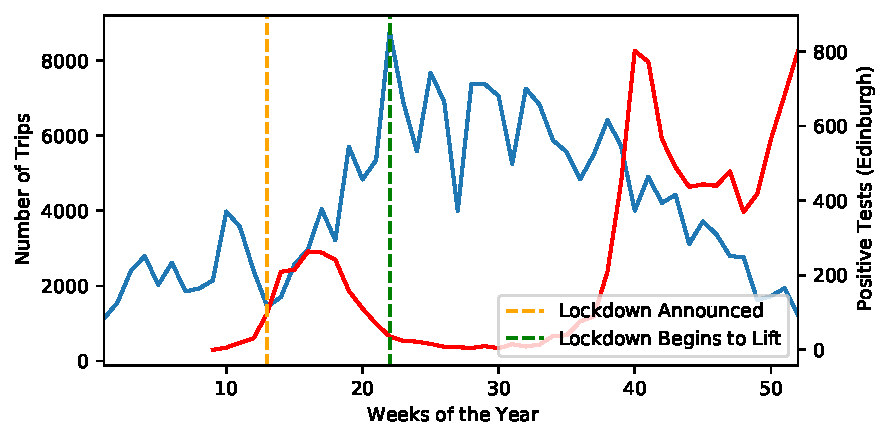
\includegraphics{report/1}
  \caption{The number of bike rides taken and the confirmed cases in 2020}
  \label{bike usage:fig:1}
\end{figure}

\begin{figure}[H]
  \centering
  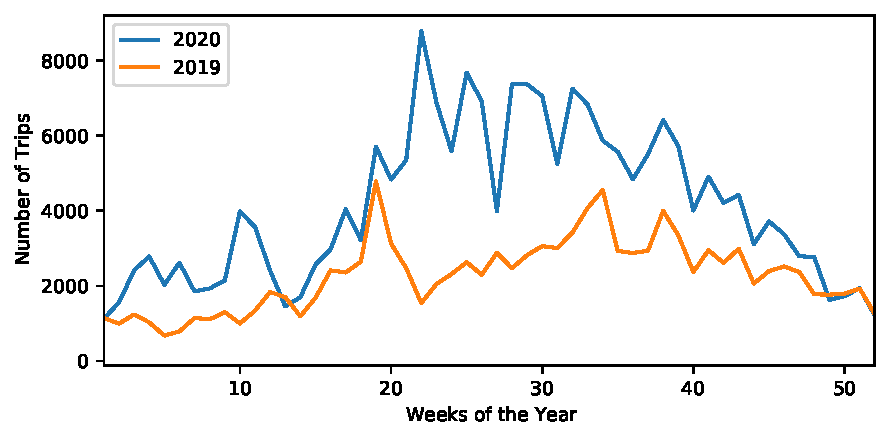
\includegraphics{report/2}
  \caption{Comparison of bikes usage in 2019 and 2020}
  \label{bike:fig:2}
\end{figure}


\paragraph{4.1.2 - Change in Purpose of Use}
Next, we hypothesised that though the trip numbers may have increased due to lockdown, the pattern of usage will have changed from commuting to use for pleasure.

We first observed a change in the popular times of usage, with the usage increase clustered towards the afternoon (figure \ref{time:fig:4}). This could be the influx of new users who are using the bikes for exercise over commuting. Indeed, when diving deeper into the usage per trip, there is a significant increase in longer trips, while shorter trips decline (figure \ref{duration:fig:6}), especially when taking into consideration the increase in the number of trips in total. We applied a T-Test to confirm our findings, using our control of 2019 and obtained a p-value < 0.05. This allowed us to reject the null hypothesis of there being no change in the average trip duration.

Furthermore, when looking at where bikes are returned (figure \ref{returnedbikes:fig:3}), we observe that percentage of bikes returned to the same station has more than doubled compared to last year (12\% to  26\%), further indicating a significant shift toward an alternative use over commuting, possibly due to people working from home.


\begin{figure}[H]
  \centering
  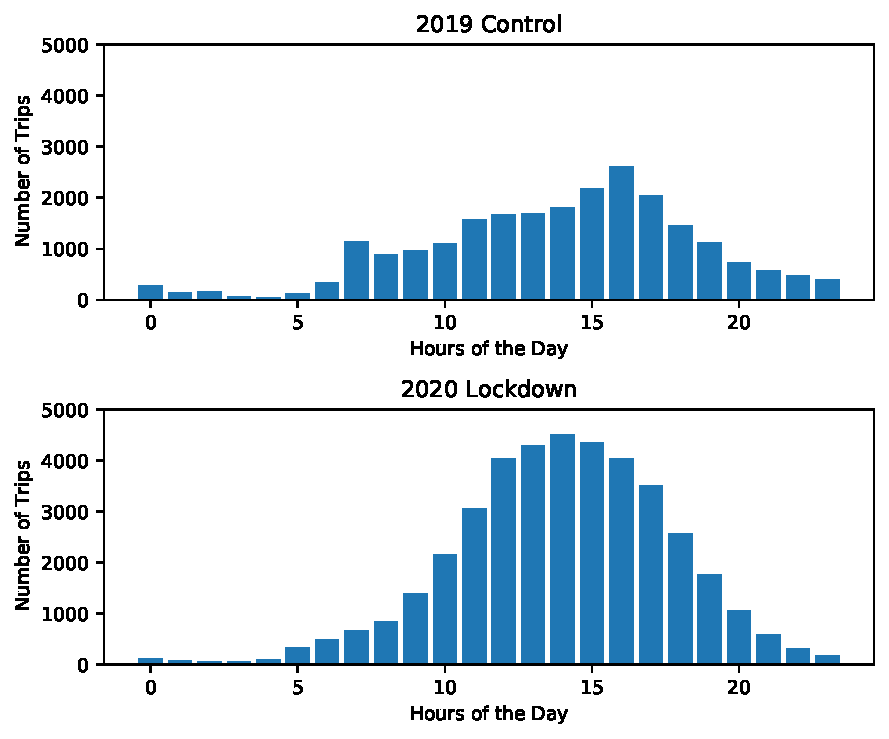
\includegraphics{report/4}
  \caption{Number of bike rides at different times of the day, comparing the same time stamp in 2019 (as a control) and 2020 during lockdown period}
  \label{time:fig:4}
\end{figure}

\begin{figure}[H]
  \centering
  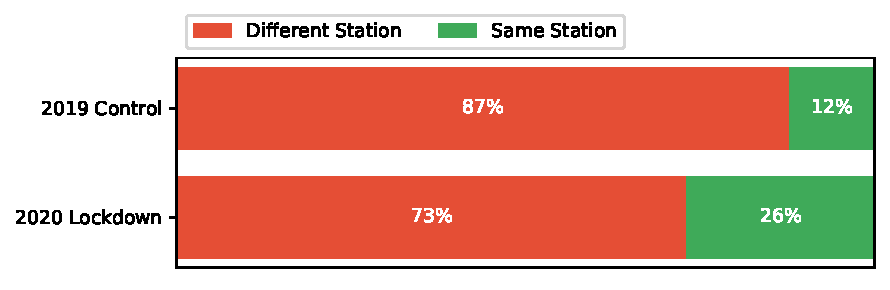
\includegraphics{report/3}
  \caption{\% of where the bikes are returned (same station they picked the bike or a different station), again comparing 2019 and 2020}
  \label{returnedbikes:fig:3}
\end{figure}

\begin{figure}[H]
  \centering
  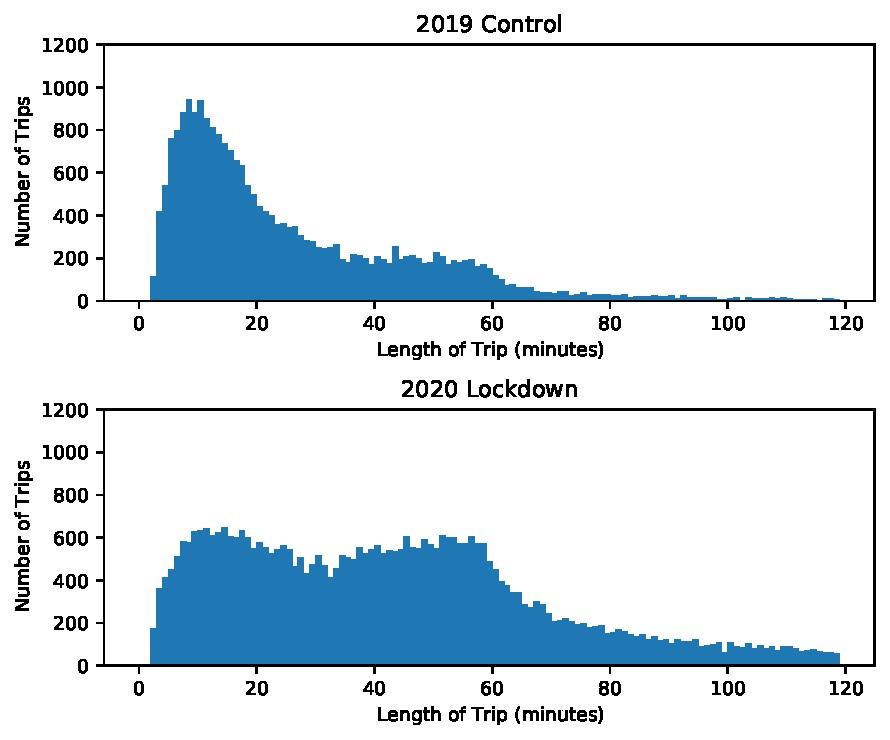
\includegraphics{report/6}
  \caption{Distribution of the trip duration, comparing 2019 and 2020}
  \label{duration:fig:6}
\end{figure}



\paragraph{Exploration - 4.1.3 - Change in Popular Areas and Routes}
Another finding was how the immediate usage of stations had changed when the pandemic arrived. Looking at figures \ref{map1:fig:7.1} and \ref{map2:fig:7.2}, we can clearly see the shift of bike usage from the areas predominantly of students/tourists to residential/scenic, i.e. out of the city centre. 
Looking at table \ref{station:table:1} we see that the most popular start stations changed from near the Meadows, to Leith, Portobello and most notably Cramond, which had very little use beforehand. A possible reason would be that as the exodus of students occurred, popularity increased in residential and less crowded areas, so people could observe social distancing and use bikes for pleasure or exercise. In particular, as stations like Cramond are relatively isolated, their main usage has not been for short commutes. This is asserted with our finding that 40\% of trips which began there to also end there, compared to 9\% at Bristo Square before lockdown.

In our statistical analysis we combined the stations that are within a 2.5 km radius from the University of Edinburgh as “city-centre stations” due to the high concentration of students and combined the other stations as “suburban stations” to be able to reason about the change in location of usage of bikes during lockdown. We noticed that previously 'city-centre' rides made up 75\% of the total rides, while during lockdown it was down to only 35\%. 

We then calculated the ratio \[ \frac{number \; of \; rides \; per \; week \; near \; city \; centre}{number \; of\; rides \; per \; week \; in \; the \; suburbs} \] giving us continuous numeric data for a specific time-frame (pre-lockdown and during lockdown period), we then applied a T-Test on the values and obtained a p-value of < 0.001, which shows a significant difference in their means. 

\begin{figure}[H]
  \centering
  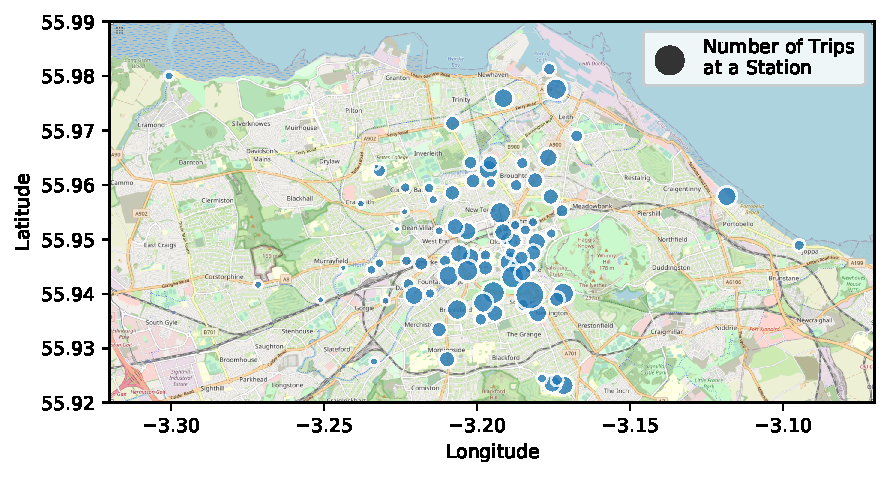
\includegraphics{report/7.1}
  \caption{Popular start/end Stations before lockdown. (Base map and data from OpenStreetMap and OpenStreetMap Foundation)}
  \label{map1:fig:7.1}
\end{figure}

\begin{figure}[H]
  \centering
  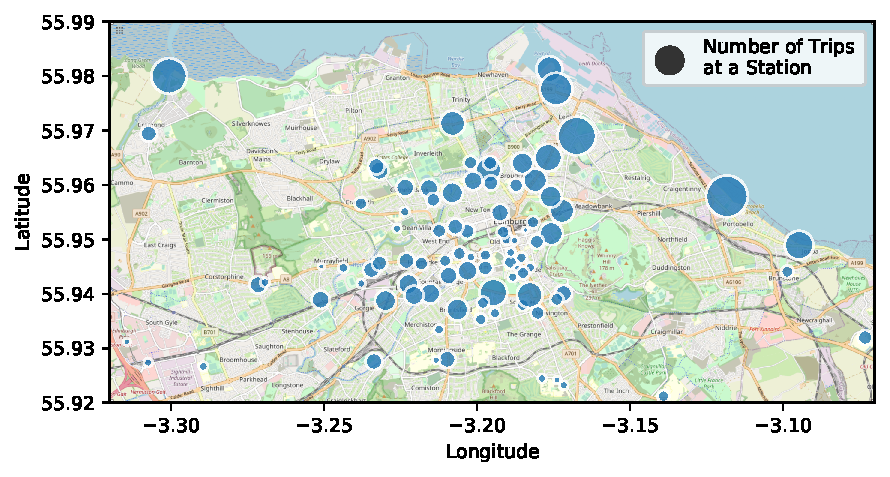
\includegraphics{report/7.2}
  \caption{Popular start/end stations during lockdown. (Base map and data from OpenStreetMap and OpenStreetMap Foundation)}
  \label{map2:fig:7.2}
\end{figure}


\begin{table}[H]
\caption{Most popular stations before and during lockdown, and the distance from the "city-centre"}
\centering
\label{station:table:1}
\begin{tabular}{llllll}
\toprule
\hline
\multicolumn{3}{c}{\textbf{Before Lockdown}} & \multicolumn{3}{c}{\textbf{During Lockdown}}    \\ \midrule
\hline
\textbf{Station Name} & \textbf{Rides} & \textbf{Distance/km} & \textbf{Station Name}   & \textbf{Rides} & \textbf{Distance/km} \\
Bristo Square     & 1847       & 3.13        & Portobello - Kings Road & 2269       & 8.03     \\
Meadows East      & 1486       & 0.86        & Duke Street             & 1816       & 3.68     \\
St Andrew Square  & 1413       & 1.24        & Cramond Foreshore       & 1655       & 13.00    \\
Portobello        & 1391       & 8.16        & Victoria Quay           & 1408       & 4.08     \\
George Square     & 1219       & 0.15        & Meadow Place            & 1208       & 0.73     \\ \bottomrule
\hline
\end{tabular}
\end{table}



\paragraph{Exploration - 4.2 - Seasonality}

To determine the effects of seasonality we mainly were interested in the difference in usage between winter and summer in 2019. When analysing the usage during the week, we were unable to notice a significant change in the distribution, but observed that weekend usage was lower in winter (figure \ref{bar:fig:5}), indicating that there are less rides for non-commuting purposes occurring then. Though there is the clear observation that in winter the mean bike rides per week is 1650 while in summer it’s 2760. Furthermore, the pattern of usage remains similar with the most popular stations not changing much. We next applied linear regression (figure \ref{linreg:fig:8.1}). This is not to predict the exact usage per day, but to determine the relationship between the weather and weekly number of trips in the given period of time. We found that predicting with average temperature as our dependent variable  obtained an adjusted $r^2$ of 0.427. Other factors such as rain and wind did not significantly improve the result, but using log of the trip number improved it to 0.48, due to the large scale difference. While this is not the greatest value, we believe it to be acceptable as it is regarding human behaviour and a single predictor variable. Indeed, we find that our residuals are not as ‘random’ as would be expected in a linear regression model, as we could observe a pattern in them. Despite of this, we do still see a clear trend that bike usage is more popular when the weather is warmer, and in general this is the clear difference between summer and winter.

\begin{figure}[H]
  \centering
  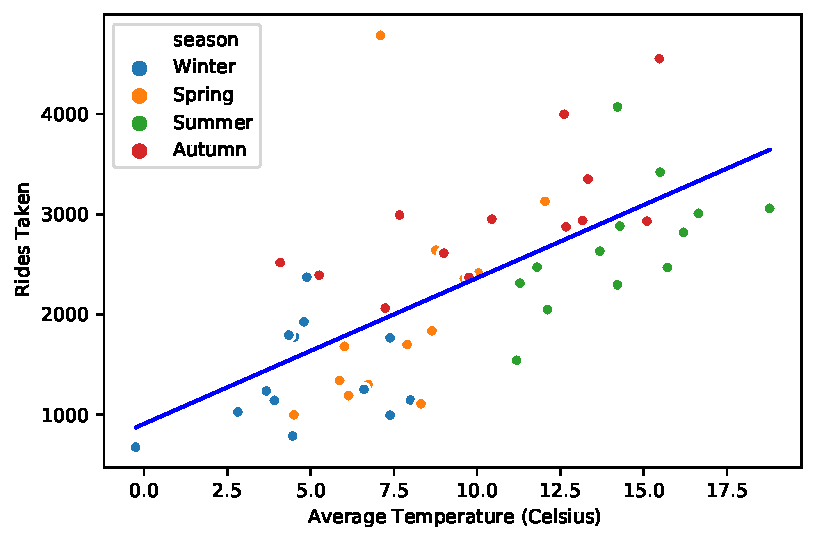
\includegraphics{report/8.1}
  \caption{Linear regression of the number of rides taken against the average temperature per week}
  \label{linreg:fig:8.1}
\end{figure}


\begin{figure}[H]
  \centering
  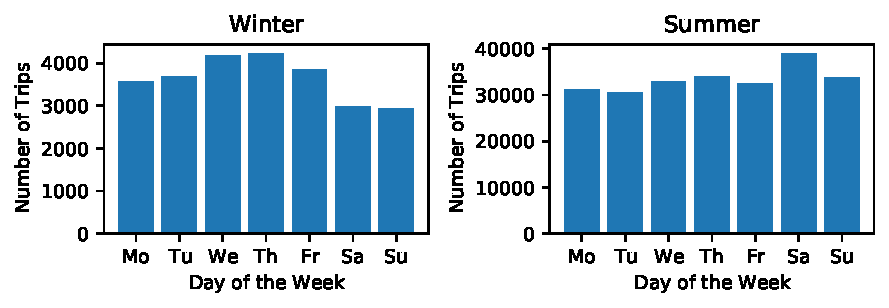
\includegraphics{report/5}
  \caption{Popular days of the week in winter vs summer during 2019}
  \label{bar:fig:5}
\end{figure}

We next use inferential statistics to determine whether these effects are statistically significant, and not by chance. We applied bootstrap to the linear regression and obtained value beta0 of ( 636.19, 1187.34) with 80\% CI and a standard error of 230.76, and value beta1 of  (105.93, 187.62) with 95\% CI and a standard error of 20.47. The p-values obtained are also < 0.001, which allows us to reject the null hypothesis that there is no significant relationship between number of trips and temperature.



% 'b' means "try to position at the bottom of the page"


\section{Discussion and conclusions}
% Suggested 400 words.

\paragraph{Comparison with any other related work}
As mentioned,  there were other similar reports conducted in New York City \cite{TEIXEIRA2020100166}, London \cite{Bike-Association} and other US cities. Interestingly, in all cases the number of bike rides decreased, while our work showed the opposite effect in Edinburgh. It must be taken into consideration the population variations between a smaller city like Edinburgh, to one magnitudes larger like New York City. However, we think this could be attributed to bike-sharing being concentrated in large areas (relative to Edinburgh) full of non-permanent residents like workers who left in droves during the State’s ‘stay at home’ order  \cite{NewYork}. This would be similar to the student areas we observed having less usage comparatively during lockdown.

\paragraph{Evaluation of own work: strengths and limitations}
It was difficult choosing which dates we would use as comparison, as we had to account for seasonal variances and we only had one previous full year of data which affected our confidence in our statistical analyses. This is because in other cities, bike-sharing is more well-established while being relatively new in Edinburgh.

We had more statistics and graphs that could be shown here that would help in explaining a better story, but were constricted by the 8 page limit. We think we have done a good job in identifying the main factors which emphasise the effects of lockdown, and our main strength was in making compelling visualisations which make it easy to grasp the magnitude of these changes (when compared to before the pandemic).

\paragraph{Improvements and extensions}
As noted our linear regression model was limited to seasonality, due to the limited data we had available. To improve and extend we would include data about the number of registered users, holidays and usage of public buses to create a better prediction model of demand. This could also be used to identify areas where more stations are needed. We would have also liked to explore the routes people took, especially when they just returned to the same station as they began, but we lacked this data. Furthermore, we also had trouble applying statistical techniques to prove the pandemic had an effect on the number of trips taken. 

\paragraph{Summary of findings}
To conclude, we were able to identify many changes in the way people used bike-sharing in Edinburgh. Though it would have been expected for usage to decline with lockdown orders and hygiene concerns, especially as COVID-19 can survive on certain surfaces for up to nine days. Nevertheless, this boom in usage shows the importance of these bikes to the people of Edinburgh to exercise or enjoy themselves during the pandemic, not just for their use in commuting. Alongside identifying how seasonal changes (towards warmer) can correlate to increased usage. We also believe that this increase would be seen in personal bike usage as an escape from lockdown and confinement at home. This is strengthened with patterns we have observed like the increased average trip duration, showing a decrease in commuting use. Furthermore, we have seen significantly more usage in stations which are further away and more sparsely located. While these could have just been longer trips, as we saw an increase in returns to the same station, we determined this to be people doing more round-trips for leisurely purposes.

\newpage

\bibliographystyle{plainurl}
\bibliography{fds-project}
\end{document}
